%%=============================================================================
%% Evaluatie casus
%%=============================================================================

\chapter{Evaluatie casus}
\label{ch:evaluatie-casus}

Hier zal bekeken worden als Elastic stack voldoet aan de vooropgestelde eisen in de casus.
Zowel de voor- als nadelen zullen aan bod komen en enkele eventuele alternatieven. Het is de bedoeling een duidelijk beeld te schetsen van de sterktes en zwaktes van Elastic stack.
Deze evaluatie gebeurde samen met Dhr. Van Den Abeele van oXya.

\section{Nodige kennis}
\label{sec:nodige-kennis}
	
Om dit te testen werd een werknemer van het bedrijf Oxya gevraagd enkele handelingen uit te voeren.
Hij kreeg daarvoor de hoofdstukken Logstash, Elasticsearch en X-Pack en Kibana ter beschikking en de mogelijkheid om via het internet te zoeken. 
Er werd ook telkens op voorhand een schatting gemaakt van de benodigde tijd.
De werknemer werd het volgende gevraagd:
\begin{enumerate}
    \item schrijf een config file voor logstash voor het lezen van een Linux syslog (2h),
    \item zoek in Elasticsearch op hoeveel logs er het laatste uur waren met het woord "sap"  in de message (30min),
    \item maak een grafiek die het aantal logs met een "word" field per tijd terug geeft (10min),
	\item intreperteer uit een gegeven dashboard wanneer iets is fout gelopen (2min). 
\end{enumerate}

1. 	De werknemer nam eerst snel het hoofsdstuk Logstash eens door. Daarna werd gekeken hoe hij de file kon normaliseren. 
Eenmaal dat beslist was, ging hij aan de slag met de input. Aangezien het path gegeven was, was de input correct geschreven op 2 minuten. Aangezien op voorhand goed nagedacht was hoe de normalisering moest gebeuren, ging het schrijven van het grok pattern ook vlot.
Als output werd std out gebruikt en Elasticsearch. Dit stond goed beschreven en was snel correct geschreven. 
Bij het eerste keer runnen van de config file werd gezien dat de datum nog niet juist was en er ook nog fields te veel waren. 
Het juist krijgen van de datum vergde nog wat extra tijd. Het verwijderen van de overbodige fields was dan weer heel snel gebeurd.

Om een volledig werkende config file te maken, zonder externe hulp, heeft het 1 uur en 6 minuten geduurd.

2. Ook hier ging de werknemer niet direct over tot de actie, maar nam eerst zijn tijd om bijpassend hoofdstuk door te nemen. 
Daarna heeft hij twee afzonderlijke queries geschreven die afzonderlijk bleken te werken na enkele pogingen. Na was prutsen met alle haakjes werden de twee queries samengebracht en dit gaf het gewenste resultaat in net geen 23 minuten.

3. Toen de werknemer niet direct een sectie zag over een grafiek maken, ging deze direct over naar de praktijk. Aangezien de symbolen duidelijk zijn, werd op geen tijd gevonden waar hij de juiste grafiek kon maken.
Een grafiek die het volledige aantal logs per tijd weergaf, ontstond in minder dan 5 minuten. Daarna kwam de moeilijkheid om enkel de logs te tonen met het "word" field. 
De werknemer werd nog enkele minuten gegeven waarin hij verschillende settings aanpaste. Na twaalf minuten was de gewenste grafiek nog niet in orde en werd de opdracht gestopt.

4. De werknemer kon na wat inzoomen op de grafieken tot op de minuut zeggen wanneer het was fout gelopen. Hij zei ook nog dat deze opdracht wel erg makkelijk was.
	

Hieruit wordt besloten dat het aanleren van de Elastic stack vlot verliep. Zeker de meest gebruikte stap, het gebruik van het dashboard, werd aangegeven makkelijk te zijn.
Vermeld moet wel worden dat gebruik gemaakt werd van enkele goed gekozen grafieken die problemen snel terug geven. 
Aangezien het maken van een speciale grafiek niet zo eenvoudig bleek te zijn werd een extra sectie geschreven. 
	
\section{Autonomie}
\label{sec:autonomie}	
	
De Elastic stack kan autonoom werken en zal alerts genereren zonder dat daarvoor iets extra hoeft gedaan te worden. 
Het is natuurlijk wel aan de eindgebruiker om te zorgen dat de grafieken en alerts relevant blijven. Dit zal dus nu en dan wat tijd vergen, maar dit zal eerder beperkt zijn. 
Na de ontwikkeling kan gesteld worden dat Elastic stack autonoom zal werken en een probleem live kan gaan alerten. 
	
	
\section{Hardware vereisten}
\label{sec:hardware-vereisten}
	
Belangrijk om mee te beginnen is dat na de installatie geen restart nodig is. Restarts worden zoveel mogelijk vermeden omdat de klant dan al zijn processen moet stoppen en dit voor overlast zorgt.

Aangezien deze bachelorproef slechts een proof of concept is, werd alles dan ook enkel geïmplementeerd op een testserver. Op deze testserver kon wel het cpu gebruik geobserveerd en geëvalueerd worden. 
Er bestaat een programma, Metricbeat genaamd, dat systeeminformatie opvraagt. Metricbeat kan op enkele minuten tijd met Elastic stack verbonden worden. Online kan een default dashboard gevonden worden die de systeem info weergeeft. Dit leek een heel eenvoudige manier om uit te vinden hoeveel cpu elk onderdeel gebruikte. Helaas valt alles onder de noemer java en wordt dan ook zo getoond.
In \ref{fig:java} werden alle java processen samen gemonitord voor 24 uur. 

\begin{figure}[h]
	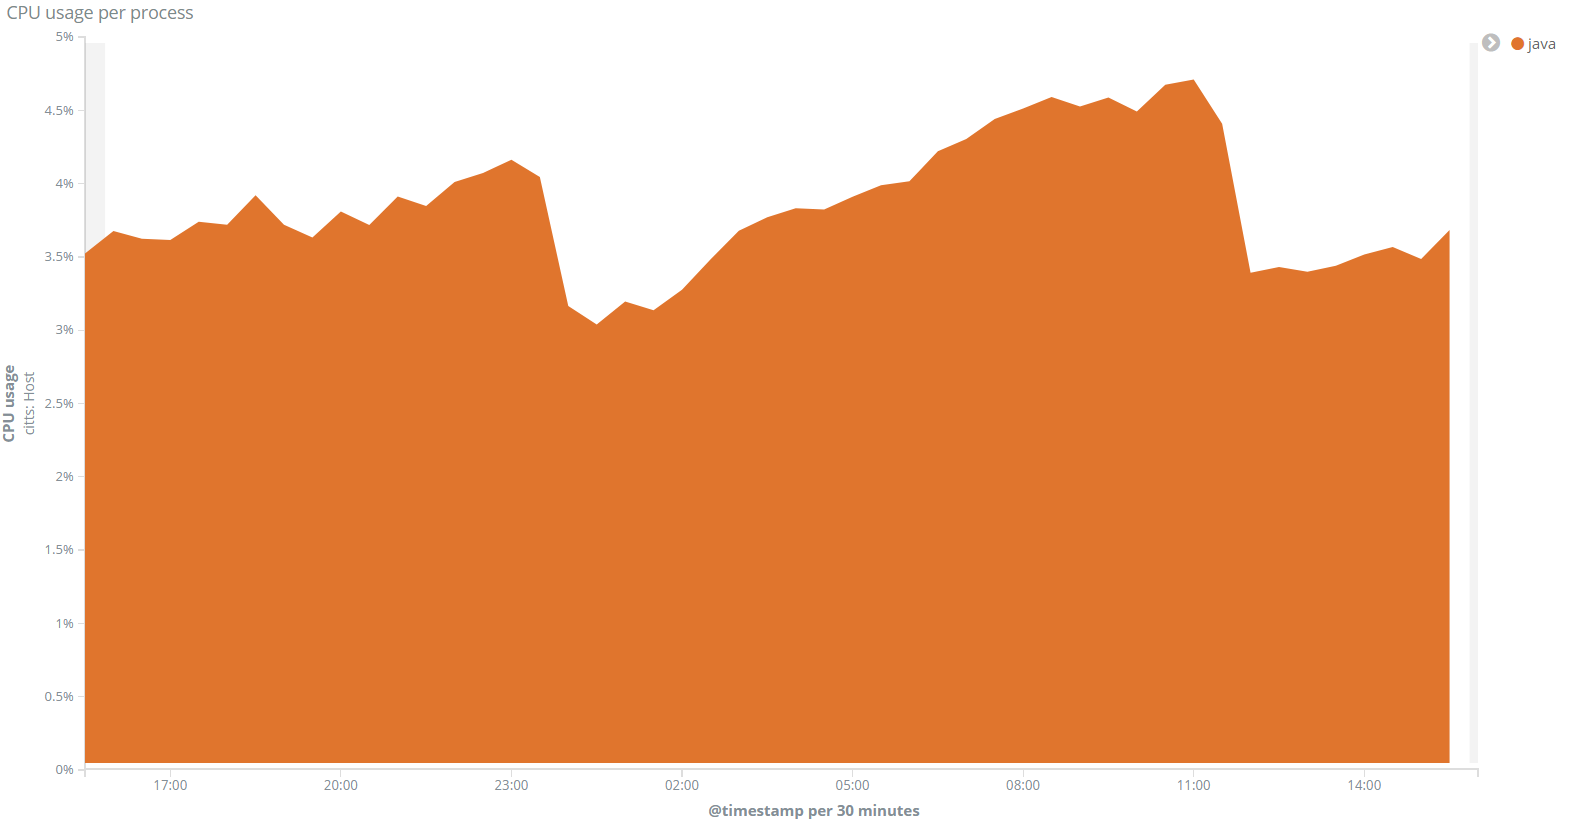
\includegraphics[width=16cm]{img/java1}
	\caption{CPU gebruik van java over 24 uur.}
	\label{fig:java}
\end{figure}

Om dus te weten hoeveel nu echt naar de Elastic stack gaat, moet ook het cpu gebruik voor java gemeten worden als Elastic stack af staat.
Als Elastic stack uitgezet wordt, kan deze monitoring niet gebruikt worden. 
Daarom werden enkele steekproeven uitgevoerd en bleek dat java dan gemiddeld 1.7\% van de cpu gebruikt. Dus de Elastic stack gebruikt gemiddeld 2\% van de cpu op de testserver. 
De testserver is dan ook nog eens veel lichter dan de servers bij de klanten.
Dit zorgt ervoor dat een klant amper een verschil in cpu gebruik zal waarnemen door het implementeren van een Elastic stack.


Voor de disk space werden enkele berekeningen uitgevoerd. Als basis werd het gebruikte geheugen en het aantal elementen bekeken. Om dit te vinden gebruikten we volgend commando in de commandline:
\lstset{escapechar=@,style=customc}        
\begin{lstlisting}[frame=single]  
	curl -XGET 'http://localhost:9200/_nodes/stats'
\end{lstlisting}
Hieruit werd gevonden dat de testomgeving reeds 3502 elementen in de Elasticsearch heeft opgeslagen. Deze elementen zouden 1.968.548 bytes innemen.
Dit zou willen zeggen dat één JSON-lement dus ongeveer 562 bytes in beslag neemt.
De testomgeving bevat een voldoende groot aantal en variatie aan elementen om deze gegevens als representatief te beschouwen voor verdere berekeningen.
Daarna werd uitgezocht hoeveel elementen grote bedrijven als Stapels en Bekaert zouden hebben op één maand. Om dit te doen werden het aantal loglijnen geteld en gekeken over welke periode deze geproduceerd werden.
Indien de log slechts de laatste 24 uur bijhield werd een gemiddelde van drie verschillende dagen genomen. 

Staples (Linux)
\begin{itemize}
	\item syslog:  10.603 elementen/dag
	\item oracle: 280.322 elementen/40 dagen
\end{itemize}	

Bekaer (Windows)
\begin{itemize}
	\item syslog: 314.044 elementen/270 dagen
	\item MySQL:   30.891 elementen/175 dagen
\end{itemize}

Voor Staples zou dit betekenen dat er elke maand 528.331 elementen bijkomen. Dit komt overeen met 296.922.022 bytes of 297MB.
Bij bekaert zou een maand slechts 40.190 elementen bevatten. Dit komt dan weer overeen met 22.586.780 bytes of 22.5MB.

Er kan dus besloten worden dat, voor het beperkt aantal log files die voor deze casus bijgehouden worden, de nodige hoeveelheid disk space erg beperkt blijft. 
Ook valt op dat een windowsserver nog minder aan disk space zal in nemen dan een linuxserver.

\section{Flexiebel}
\label{sec:flexiebel}

oXya heeft geen vaste pakketten. Het maakt aanbiedingen op maat van elke klant. Hierdoor zitten ze dus met verschillende besturingssytemen en databanken.
Als besturingssystemen werden redhat en windows server 2012R2 getest. En als databases werden oracle en MySQL bekeken.
De config files zijn terug te vinden in \ref{ch:appendix}. 
Deze config files kunnen dus voor elk type logfile geschreven worden. Er is wel een verschil in hoe ver een file genormaliseerd kan worden.
Een oracle file zal voorbeeld verder genormaliseerd kunnen worden dan een MySQL file. Dit zal voor MySQL de monitoringmogelijkheden beperken.
Maar er kan dus gesteld worden dat het flexibel genoeg is aangezien het eender welke log files kan gebruiken als input data.


\section{Annomaly detectie}
\label{sec:annomaly detectie}

oXya zou graag op de hoogte gebracht worden als er zich ergens uitzonderlijk gedrag voor doet. De mogelijkheid is er om statische thresholds te plaatsen.
Maar in plaats daarvan wordt gekozen om te werken met dynamische thresholds. Dit om te verkomen dat bij een groeiend bedrijf telkens de waarden aangepast moeten worden.
In \ref{subsec:timelion} zal bekeken worden wat de mogelijkheden zijn met de vrijheid die daar gegeven wordt.
In \ref{subsec:machine-learning} daarentegen is de vrijheid beperkt, maar indien het van genoeg input voorzien wordt, is het zeker betrouwbaar.

De servers die oXya monitort zijn meer belast in de week dan in het weekend. Ook overdag is er meer activiteit dan 's nachts. Het ideale zou dus zijn om te gaan vergelijken met hetzelfde moment in de voorbije weken \autocite{hourweekanalyse}.

Over het algemeen beschikt Elastic stack dus over enkele nuttige anomaliedetectie mogelijkheden. 
Er is een breed aanbod en afhankelijk van de toepassing zal dus een gepaste anomaliedetectie gekozen moeten worden.

\subsection{Timelion}
\label{subsec:timelion}

Eén van de mogelijkheden is om de gegevens van dit moment te gaan vergelijken met het gemiddelde $\pm$ 3 keer de standaard deviatie van de voorbije waarden.
Dit zou willen zeggen dat met een 99,7\% zekerheid gezegd zou kunnen worden als een waarde uitzonderlijk is of niet. Om het gemiddelde en de standaard deviatie te berekenen zullen de waarden van de laatste 24 uur gebruikt worden. 
In deze situatie worden beste resultaten verkregen als de waarden per uur gegroepeerd worden. Om deze grafiek te creëren dienen volgende commando's uitgevoerd te worden:
\lstset{escapechar=@,style=customc}        
\begin{lstlisting}[frame=single]  
	.es(index="mssql").label("Values"),
	.es(index="mssql",offset=-1h).movingaverage(10).max(15).sum(.es(index="mssql",offset=-1h).movingstd(10).multiply(3)).label("gem + 3std"),
	.es(index="mssql",offset=-1h).movingaverage(10).max(15).sum(.es(index="mssql",offset=-1h).movingstd(10).multiply(-3)).label("gem - 3std")
\end{lstlisting}

\begin{figure}[h]
	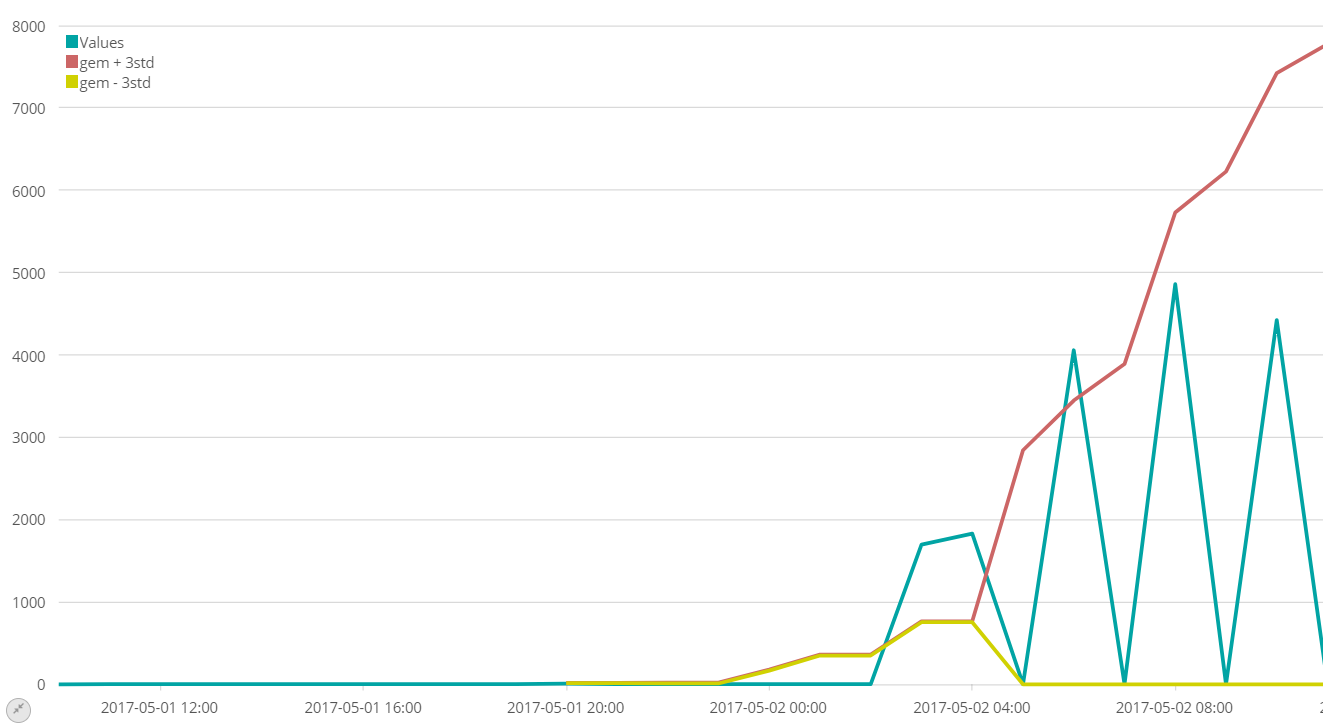
\includegraphics[width=16cm]{img/avg3std}
	\caption{Anomaliedetectie aan de hand van het gemiddelde en de standaard deviatie.}
	\label{fig:avg3std}
\end{figure}

De grafiek van dit moment moet zich dus tussen de andere twee grafieken bevinden anders dient er een alert opgesteld te worden voor een anomaly.


Een andere mogelijkheid met timelion is de implementatie van het holt-winter algoritme \autocite{holtwinters}.
Ook dit heeft zijn voor- en nadelen. Het zal meer rekening gaan houden met de trend van de grafiek. Het enige probleem hiermee is dat er nog geen betrouwbaarheidsintervalen geïmplementeerd zijn.
Wat wel een mogelijkheid zou zijn is dat de grafiek zich tussen 0,5 en 1,5 keer de verwachte holt-winter waarde moet bevinden.
\lstset{escapechar=@,style=customc}        
\begin{lstlisting}[frame=single]  
	.es(index="mssql").label("Values"),
	.es(index="mssql",offset=-1h).holt(0.1,0.1).multiply(0.5).label("0.5*holt"),
	.es(index="mssql",offset=-1h).holt(0.1,0.1).multiply(1.5).label("1.5*holt")
\end{lstlisting}

\begin{figure}[h]
	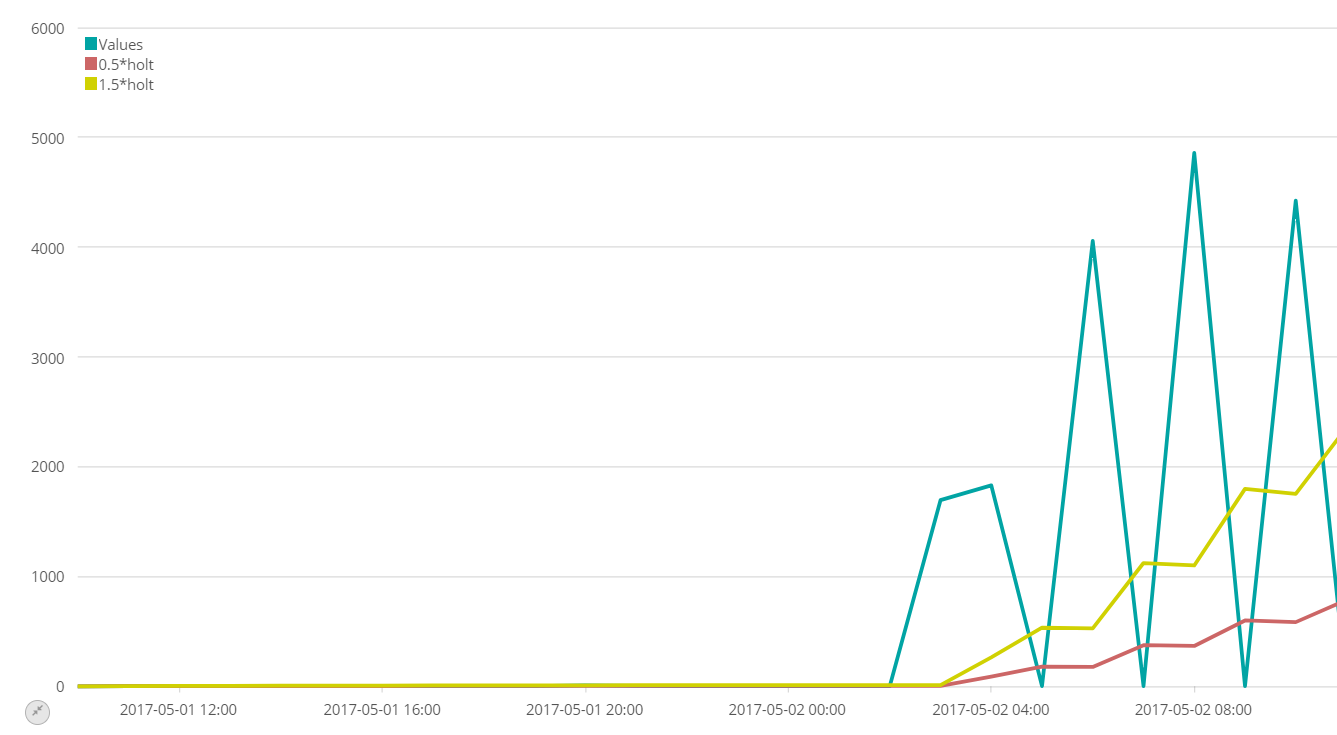
\includegraphics[width=16cm]{img/holtwinters}
	\caption{Anomalie detectie aan de hand van Holt Winters.}
	\label{fig:holtwinters}
\end{figure}


Maar ook hier is het weer mogelijk om andere dingen mee te doen door een combinatie te maken met andere mogelijkheden.
Hier zijn dus heel wat mogelijkheden en de uitkomst zal afhangen van het gekozen algoritme. 

\subsection{Machine Learning}
\label{subsec:machine-learning}

Zoals reeds besproken is er bij Machine Learning, naast het kiezen uit de vier warnings, geen vrijheid. Maar dit hoeft ook niet, want als de juiste elementen hier als input gebruikt worden doet Machine Learning de rest. Hoe meer input Machine Learning krijgt hoe accurater er een alert gestuurd kan worden. 
Deze tool is nog in beta en heeft dus ook enkele kinderziektes. Zo werd ontdekt dat na het ontstaan van een vijftal anomanlieën op een termijn van 24 uur Machine Learning het moeilijk heeft om terug naar een stabiele toestand te gaan. Zo zou het in de daaropvolgende week mogelijk zijn dat nog grotere anomalieën niet opgemerkt worden.

Machine Learning heeft dus nog enkele minpunten, maar deze wegen niet op tegen de toch al nuttige functionaliteit.

\subsection{Eigen detectie}
\label{subsec:eingen-detectie}

Indien bovenstaande tools nog niet aan de wensen voldoen, is er nog altijd de optie om een eigen detectie tool te ontwerpen. Het ontwikkelen van een eigen detectie tool is mogelijk door gebruik te maken van de java api \autocite{javaapi}. 
Bij het ontwikkelen van een eigen detectie tool in java kan dan gebruik gemaakt worden van alle Elasticsearch queries. 
De java api zorgt ervoor dat de limiet van anomalie detectie bij jezelf ligt.

\section{Alers}
\label{sec:alerts}

De alerts die in Logstash gegenereed worden bevatten in de titel het probleem en op welke host het probleem zich stelt.
Als de e-mail dan geopend wordt, kan men terug vinden wanneer het probleem zich voor deed. Nog eens op welke machine het probleem vastgesteld werd. En dan de boodschap die bij het probleem hoort. 
Deze boodschap is voor een werknemer van oxya voldoende om te kunnen beslissen als er opvolging nodig is of niet.

Ook de alerting via Watcher kan duidelijk verlopen. Watcher biedt ook een breed gamma aan mogelijkheden aan. Door oXya werd gekozen om de alerting via email te laten verlopen.
Watcher maakt het mogelijk om te alerten op Elasticsearch queries. Maar Watcher kan ook gebruikt worden om te alerten op Timelion of op de Machine Learning.

Dus ook op gebied van alerting zijn er genoeg mogelijkheden.
